\documentclass[12pt]{article}
\usepackage[utf8]{inputenc}
\usepackage{amsmath}
\usepackage{graphicx}
\usepackage{float}
\usepackage{lineno}
\setlength{\parindent}{2em}
\setlength{\parskip}{1em}
\renewcommand{\baselinestretch}{1.2}
\newcommand\dbyd[2]{\frac{\mathrm d{#1}}{\mathrm d{#2}}}
\newcommand{\R}{\mathcal{R}}
\title{Intensional infect proportion of newborn, finding eigenvalues}

\begin{document}
\linenumbers

\maketitle

\section{Motivation}
In history, before vaccination became a developed technology, humanity has limited power when encountering viral infection. Intentional infection however, act as a precursor of vaccination, was introduced long ago. Although people did not fully understand the detailed mechanism of intentional infections before modern centuries, this method was used extensively to battle some deadly disease, smallpox as a famous representative. There are different strategies in vaccination. Some vaccinations are applied to younglings, for example, polio. Other vaccination may be applied to adults, flu vaccination is a commonly seen one. In fact, same strategies may be used in intentional infection as well.
\section{Introduction}

Primarily, there are two strategies when performing intentional infection on a population level. One is to intentionally infect newborns, since it is much easier to identify newborn individuals, in contrast with identify and intentionally infect susceptible individuals, which is our second approach. In this document, we discuss and analyze the basic modeling of our first approach.

\section{System of differential equations}
To begin with, the following assumptions are made:
\begin{itemize}
\item There is no disease induced mortality.
\item Birth and natural death rate are the same, so the total population remains constant.
\item The latent period is short enough to be ignored.
\item All susceptible individuals are equally likely to be infected, and all infected individuals are equally infectious.
\end{itemize}

With the assumptions above, we now setup our system of equations.
$S$, $I$ and $R$ represent the proportion of susceptible, infected and recovered with respect to total population.
\begin{equation}\label{1}
\begin{split}
\dbyd{S}{t}&=\mu(1-p)- \beta SI-\mu S \\
\dbyd{I}{t}&=\beta SI+\mu p-\gamma I -\mu I\\
\dbyd{R}{t}&=\gamma I-\mu R
\end{split}
\end{equation}

Here, $\beta$ is the transmission rate, $\gamma$ is the recovery rate,
$\mu$ is the \emph{per capita} rate of birth and death, $p$ is the
proportion of newborns that are intentionally infected.

For simplicity, we now convert the system into dimensionless form using dimensionless time coordinate,
\begin{equation}
\tau=(\gamma+\mu)t \,,
\end{equation}
which yields
\begin{subequations}
\begin{align}
\dbyd{S}{\tau}&=\epsilon(1-p)- \R_0  SI-\epsilon S \,,\\
\dbyd{I}{\tau}&=\R_0 SI+\epsilon p-I \,,
\end{align}
\end{subequations}
where $\epsilon=\frac{\mu}{\gamma+\mu}$, $\R_0=\frac{\beta}{\gamma+\mu}$.

\section{Endemic Equilibrium}

To find the endemic equilibrium (EE), we need to let both equations in (3) equal to 0, after solving, we get:
\begin{align}
\hat{I} &= \frac{\epsilon(\R_0 -1)+ \epsilon \sqrt{(\R_0-1)^2+4\R_0
    p}}{2\R_0} \\
\hat{S} &=\frac{1}{\R_0}-\frac{2p}{(\R_0 -1)+ \sqrt{(\R_0-1)^2+4\R_0 p}} 
\end{align}

To analyze the local stability of the EE, we need to use the Jacobian matrix,
\begin{equation}
\mathcal{J} =
\begin{bmatrix}
    \ -\R_0 I-\epsilon       & -\R_0 S \\
    \ \R_0 I       & \R_0 S-1 \\
\end{bmatrix} \,.
\end{equation}

Now for simplicity, let 
%
\begin{linenomath*}
\begin{equation}\label{E:}
K = (\R_0 -1)+ \sqrt{(\R_0-1)^2+4\R_0 p} \,.
\end{equation}
\end{linenomath*}
%
Notice, $K>0$ if $p\neq 0$.

Thus, the Jacobian evaluated at endemic equilibrium is the following:
\begin{equation}
\mathcal{J}|_{EE} =
\begin{bmatrix}
    \ -\frac{\epsilon K}{2}-\epsilon       & -1+\frac{2p \R_0}{K} \\
    \ \frac{\epsilon K}{2}       & -\frac{2p \R_0}{K} \\
\end{bmatrix}
\end{equation}

The eigenvalues of this Jacobian is:

\begin{equation}
\lambda = \frac{-(\epsilon K^2+2\epsilon K +4p\mathcal{R}_0) \pm \sqrt{(\epsilon K^2+2\epsilon K +4p\mathcal{R}_0)^2-4(2\epsilon K^3+8\epsilon Kp\mathcal{R}_0)}}{4K}
\end{equation}

If the discriminant is positive, then since
%
\begin{linenomath*}
\begin{multline}\label{}
\sqrt{(\epsilon K^2+2\epsilon K +4p\mathcal{R}_0)^2-4(2\epsilon
  K^3+8\epsilon Kp\mathcal{R}_0)} \\
 \leq \left|\epsilon K^2+2\epsilon K +4p\mathcal{R}_0\right|  \,,
\end{multline}
\end{linenomath*}
%
we can conclude that $\Re(\lambda)<0$ for all $p\neq 0$. If the discriminant is negative then $\Re(\lambda)<0$ as well.  Thus the EE is always stable.

But to fully understand the dynamics of the system, we are also interested in whether it is possible to have a complex eigenvalue, which will lead to damped oscillation. That requires us to look more closely at the discriminant of the eigenvalue.

Although it is hard to determine the sign of discriminant analytically, we can still plot the value of discriminant as a function of other parameter, i.e. $p$ or $\R_0$

\subsection{Dependence of discriminant on proportion intentionally infected ($p$)}

We will start our analysis with specific values of each parameter. Given the variolation history of smallpox, it is reasonable to use the parameters of smallpox as an example.

The following values are used (need reference): 
\begin{enumerate}
\item With 50 years of average life span, $\mu=\frac{1}{50*365}$ per day.
\item 22 days of mean infectious period, $\gamma=\frac{1}{22}$ per day.
\item $\R_0=4.5$.
\end{enumerate}
Therefore, we can calculate $\epsilon=\frac{\mu}{\mu+\gamma}=0.0012$

I plotted the discriminant with Mathematica, range of $p$ is $[0,1]$.

\begin{figure}[H]
  \caption{Plot discriminant with $p$ to be the variable.}
  \centering
  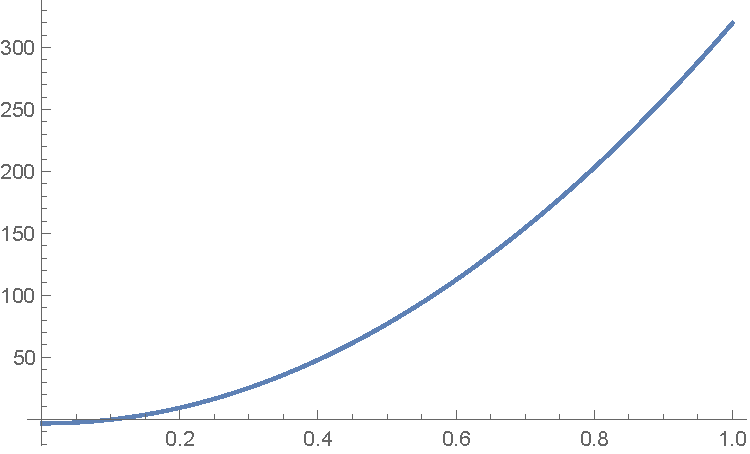
\includegraphics[width=1.1\textwidth]{Figures/Discriminant_plot_newborn.pdf}
\end{figure}

The $p$-intercept of this graph is $p=0.103995$. Meaning, with a proportion of 0.103995 or less, there is going to be a damped oscillation.

\subsection{Dependence of discriminant on basic reproduction number ($\R_0$)}
It is also interesting to investigate the effect of $\R_0$ on discriminant. Since it is often the case where people have limited resources and ability to apply such medical treatment.

Again, we take $\mu=\frac{1}{50*365}$, $\gamma=\frac{1}{22}$, $\epsilon=\frac{\mu}{\mu+\gamma}=0.0012$.

We made an array of plots by taking $p=0.1,0.2,0.3...$

\begin{figure}[H]
  \caption{Plot discriminant with $\R_0$ to be the variable.$p=0.1$, the $R_0$ -intercept is $\R_0 = 0, 5.74966$}
  \centering
  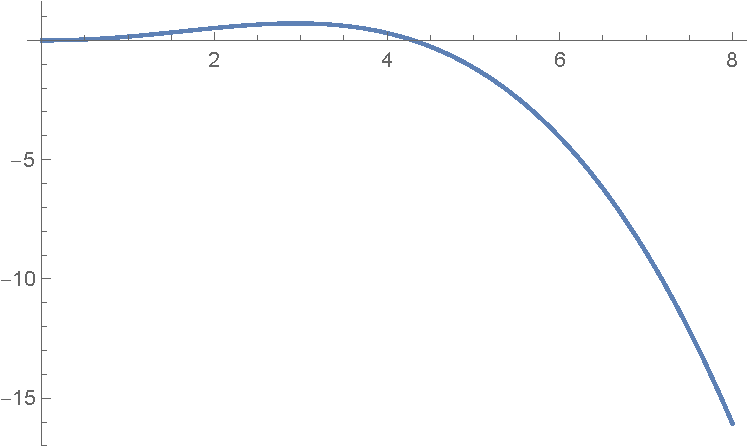
\includegraphics[width=1.1\textwidth]{Figures/Plot_R_0_p_0_1.pdf}
\end{figure}

\begin{figure}[H]
  \caption{Plot discriminant with $\R_0$ to be the variable.$p=0.2$, the $\R_0$ -intercept is $\R_0 = 0, 17.0518$}
  \centering
  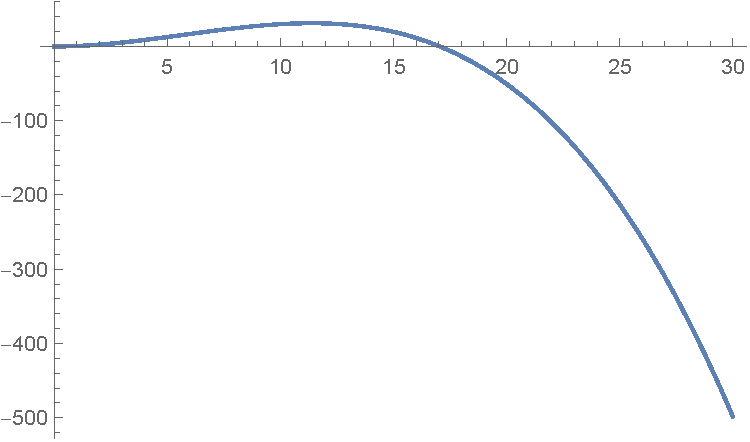
\includegraphics[width=1.1\textwidth]{Figures/Plot_R_0_p_0_2.pdf}
\end{figure}

\begin{figure}[H]
  \caption{Plot discriminant with $\mathcal{R}_0$ to be the variable.$p=0.3$, the $\mathcal{R}_0$ -intercept is $\mathcal{R}_0 = 0, 37.4537$}
  \centering
  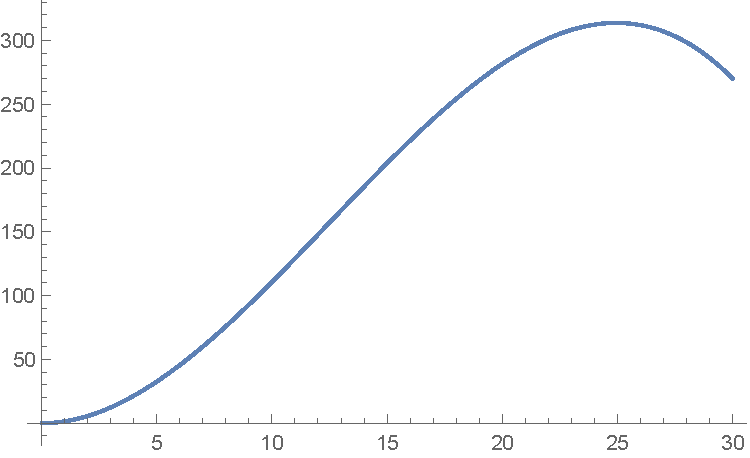
\includegraphics[width=1.1\textwidth]{Figures/Plot_R_0_p_0_3.pdf}
\end{figure}

For $p=0.4$ or higher, the graphs look similar, but with even higher value for the discriminant and larger value for $\R_0$-intercept.

Thus, it is evident that a larger $\R_0$ value will eventually lead to damped oscillation, but the threshold for this to happen increases as $p$ increases.

\section{DFE}

Disease free equilibrium is the equilibrium when there is nobody infected in the system, which means, $I=0$

Again, we solve equations (3) by letting both $\dbyd{S}{\tau}$ and $\dbyd{I}{\tau}$ equal to 0. But this time, since it is disease free, $I=0$ as well.

Thus, we obtain:
\begin{equation}
\dbyd{I}{\tau}=\epsilon p=0
\end{equation}
Since $\epsilon\neq0$, it is necessary that $p=0$. But this is the case when there is no intentional infection, and there is no solution to this system if $p\neq0$. Therefore, we can conclude that there is no disease free equilibrium(DFE) for this model if $p\neq0$

\section{I at EE}

\begin{figure}[H]
  \caption{Infected population at EE as a function of $\R_0$, blue curves are for intentional infections with $p=0.3,0.2,0.1$, from top to bottom. Orange curve is for $p=0$, which is the endemic equilibrium for basic SIR model.}
  \centering
  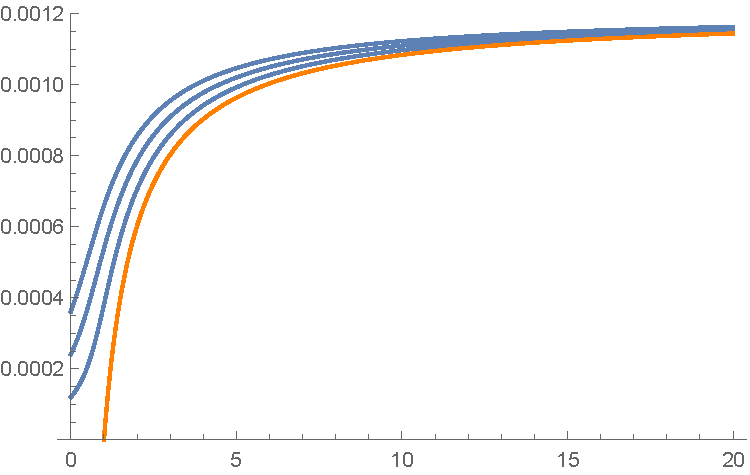
\includegraphics[width=1.1\textwidth]{Figures/I_at_E_E_SIR_vs_Int.pdf}
\end{figure}

A non-zero $p$ value will increase the proportion infected at endemic equilibrium. The amount increased has a direct relationship with $p$. 

To know how much $I|_{EE}$ has increased, it is helpful to see the ratio between different $I$ values at different $p$.

\begin{figure}[H]
  \centering
  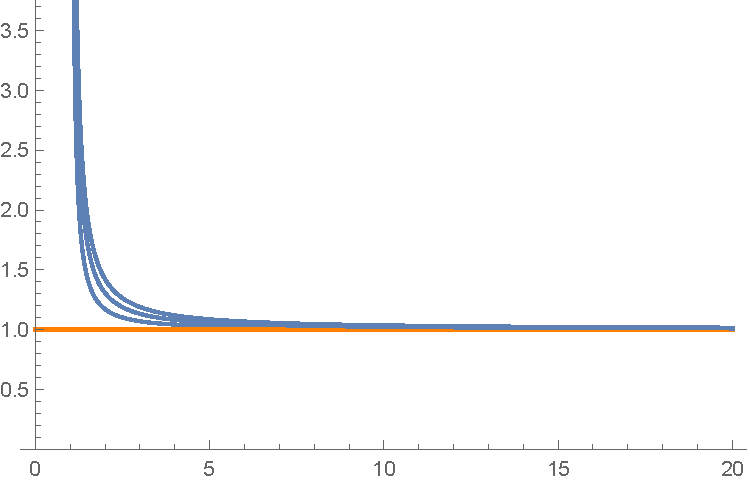
\includegraphics[width=1.1\textwidth]{Figures/I_at_E_E__Ratio_plot.pdf}
  \caption{Ratio of $I$ at EE between intentional infection cases and basic SIR model, as a function of $\R_0$, blue curves are for intentional infections with $p=0.3,0.2,0.1$, from top to bottom. Orange line is horizontal line at 1.}
\end{figure}

\end{document}
